\documentclass{standalone}    
\usepackage{pgfplots}

\begin{document}

  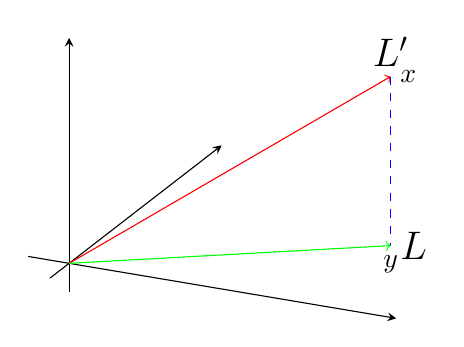
\begin{tikzpicture}
    \pgfplotsset{grid style={dashed}}
  \begin{axis}[
    axis lines=middle,samples=200,
    xmin=-0.5,xmax=4,
    ymin=-0.5,ymax=4,
    zmin=-0.5,zmax=4,
    ticks=none]
  \draw[->,solid,red] (axis cs:0,0,0) -- (axis cs:3,2,3)node[right,black]{$x$};
  \draw[dashed,blue] (axis cs:3,2,3) -- (axis cs:3,2,0);
  \draw[->,solid,green] (axis cs:0,0,0) -- (axis cs:3,2,0)node[below,black]{$y$};

  \node[above,font=\Large] at (axis cs:3,2,3) {$L'$};
  \node[right,font=\Large] at (axis cs:3,2,0) {$L$};
  \end{axis}
  \end{tikzpicture}
\end{document}
